% Created 2025-01-01 水 22:54
\documentclass[a4paper, 10pt, notitlepage, twocolumn, uplatex, oneside, dvipdfmx]{jsarticle}
\usepackage[dvipdfmx]{graphicx, color}
\usepackage{ulem}
\usepackage[utf8]{inputenc}
\usepackage{mlmodern}
\usepackage{mdframed}
\usepackage{minted}
\usepackage{natbib}
\usepackage{amsmath, amssymb, amsthm}
\definecolor{shadecolor}{gray}{0.92}
\usepackage[dvipdfmx,colorlinks=true,linkcolor=blue,filecolor=blue,urlcolor=blue]{hyperref}
\usepackage{pxjahyper}
\surroundwithmdframed[backgroundcolor=shadecolor,hidealllines=true]{verbatim}
\renewcommand{\baselinestretch}{0.86}
\setlength{\voffset}{-0.7in}
\setlength{\hoffset}{-0.5in}
\setlength{\headsep}{0cm}
\setlength{\topmargin}{-0.5cm}
\setlength{\oddsidemargin}{0cm}
\setlength{\textwidth}{525pt}
\setlength{\textheight}{46\baselineskip}
\addtolength{\textheight}{\topskip}
\author{sugayu}
\date{\today}
\title{\textbf{matplotlibで3次元図の作成}}
\begin{document}

\maketitle
\tableofcontents

\section{基準の図}
\label{sec:orgfa59f90}
\texttt{fig.add\_subplot()} に \texttt{projection='3d'} を渡して3次元図を作成する。
このとき返ってくるのは3次元専用の軸オブジェクト \texttt{Axes3D} である。

\begin{minted}[frame=lines,framesep=2mm,linenos=true,breaklines]{ipython}
from mpl_toolkits.mplot3d.axes3d import Axes3D
from sugayutils import colors

theta = np.pi / 2.0
phi = np.linspace(0.0, 2.0 * np.pi, 91)


def xyz(theta, phi):
    x = np.sin(theta) * np.cos(phi)
    y = np.sin(theta) * np.sin(phi)
    z = np.cos(theta) * np.ones_like(phi)
    return x, y, z


x, y, z = xyz(theta, phi)


def plot_fiducial(left=-0.1) -> Axes3D:
    fig = plt.figure(figsize=(3.5, 3.5))
    fig.subplots_adjust(left, 0.1, 0.98, 0.99, 0.0, 0.0)
    ax = fig.add_subplot(1, 1, 1, projection='3d')
    ax.plot(x, y, z, c=colors.black)
    ax.set_xlim3d(-1.0, 1.0)
    ax.set_ylim3d(-1.0, 1.0)
    ax.set_zlim3d(-1.0, 1.0)
    ax.set_xlabel('x')
    ax.set_ylabel('y')
    ax.set_zlabel('z')
    ax.set_aspect('equal')
    return fig, ax


def savefig(fig, fsave) -> str:
    fig.savefig(fsave)
    fig.clear()
    plt.close()
    return f'[[file:{fsave}]]'


fig, _ = plot_fiducial()
savefig(fig, './obipy-resources/fiducial_3d.png')
\end{minted}

\phantomsection
\label{}
\begin{center}
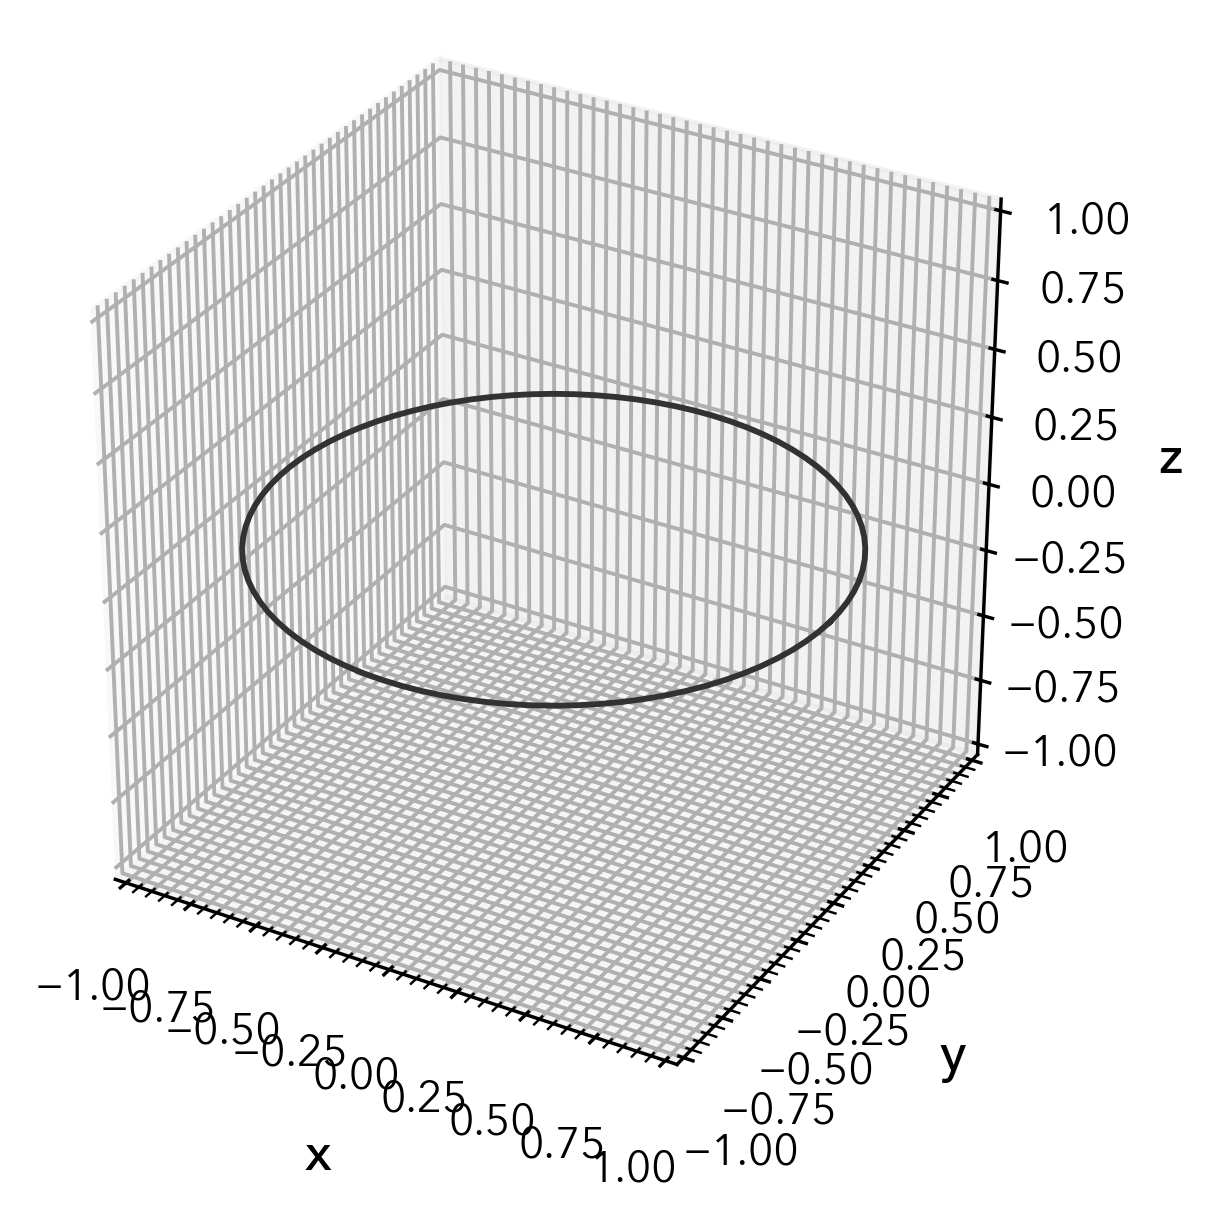
\includegraphics[width=1.0\linewidth]{./obipy-resources/fiducial_3d.png}
\end{center}

\begin{verbatim}
なお、おそらく ~Jupyter notebook~ の仕様で図の余白が自動的に調整されてしまうので、
ここでは ~ob-ipython~ のファイル保存形式ではなく、保存方法と表示方法を指定している。
ただし出力のたび、いちいち手作業が必要になる。
また、この場合の方がプロットがとても速い。
\end{verbatim}
\section{基本}
\label{sec:org1ceb77d}
\subsection{面をプロット}
\label{sec:org3dfa4fd}
\begin{minted}[frame=lines,framesep=2mm,linenos=true,breaklines]{ipython}
fig, ax = plot_fiducial()
theta = np.linspace(0.0, np.pi / 2.0, 9).reshape(-1, 1)
_xyz = xyz(theta, phi)
ax.plot_surface(
    *_xyz,
    color=colors.sky,
    # facecolors=facecolor,
    alpha=1.0,
    # shade=True,
    # lightsource=light,
)
savefig(fig, './obipy-resources/surface_3d.png')
\end{minted}

\phantomsection
\label{}
\begin{center}
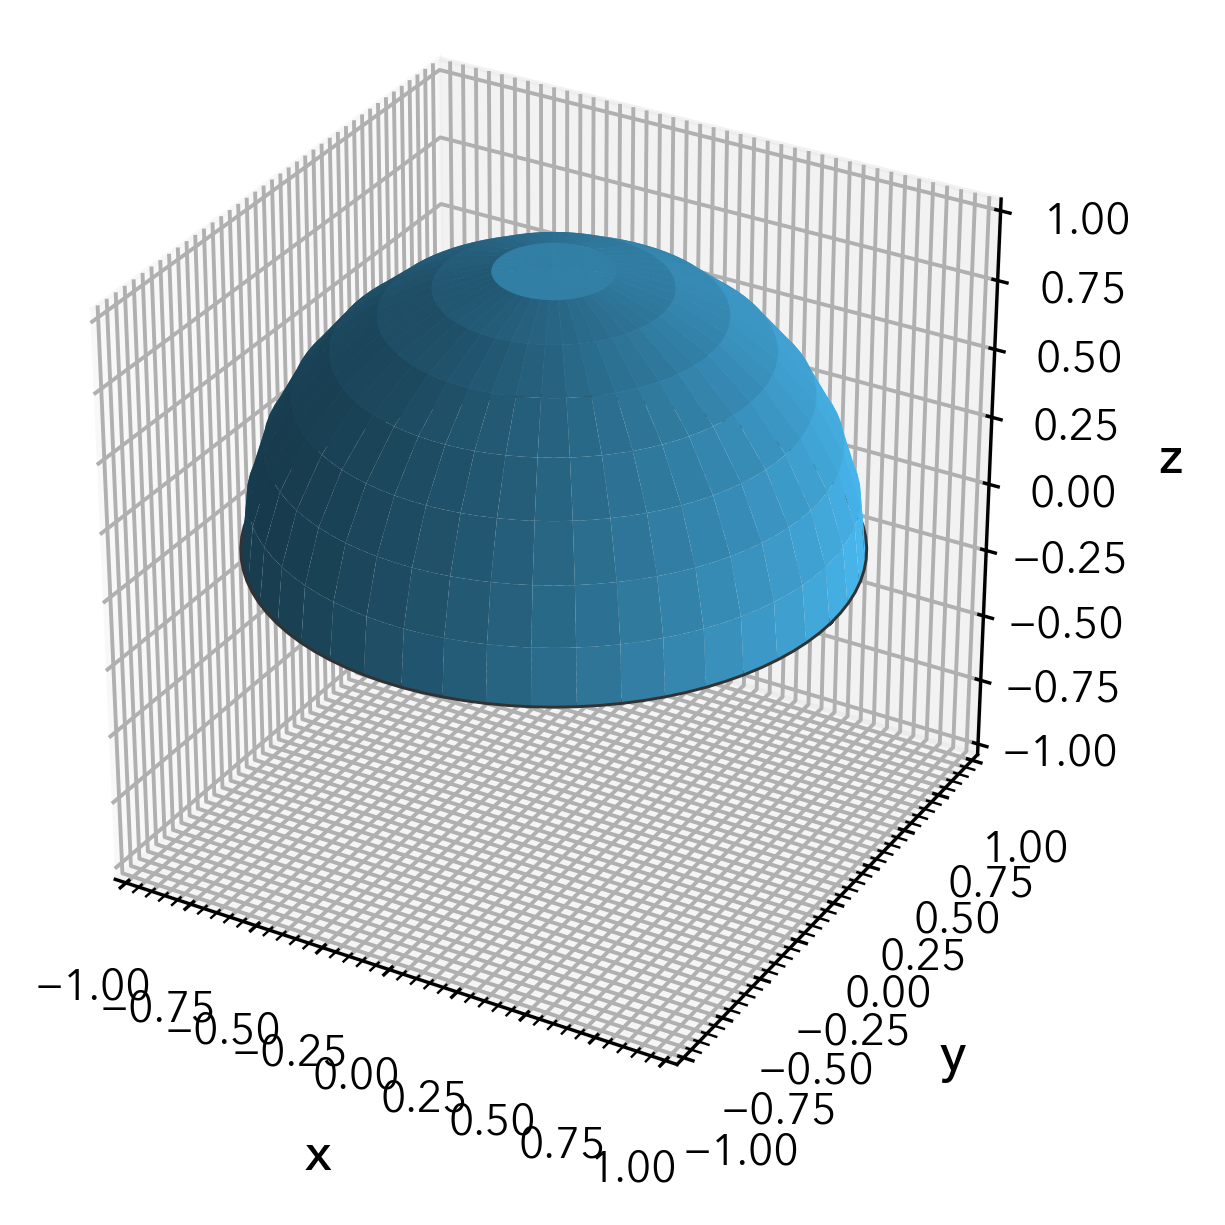
\includegraphics[width=1.0\linewidth]{./obipy-resources/surface_3d.png}
\end{center}

光が当たる角度は引数の \texttt{lightsource} に \texttt{matplotlib.colors.LightSource} を入れて指定できる。
詳しくは
\section{軸の設定}
\label{sec:org64c14f3}
\subsection{ズーム}
\label{sec:org99ba930}
ズームをする関数は用意されていない。
軸の表示範囲を調整して似た機能を実現する。
\begin{minted}[frame=lines,framesep=2mm,linenos=true,breaklines]{ipython}
fig, ax = plot_fiducial()
zoom = 1.3
ax.set_xlim3d(np.array(ax.get_xlim3d()) / zoom)
ax.set_ylim3d(np.array(ax.get_ylim3d()) / zoom)
ax.set_zlim3d(np.array(ax.get_zlim3d()) / zoom)
savefig(fig, './obipy-resources/zoom_3d.png')
\end{minted}

\phantomsection
\label{}
\begin{center}
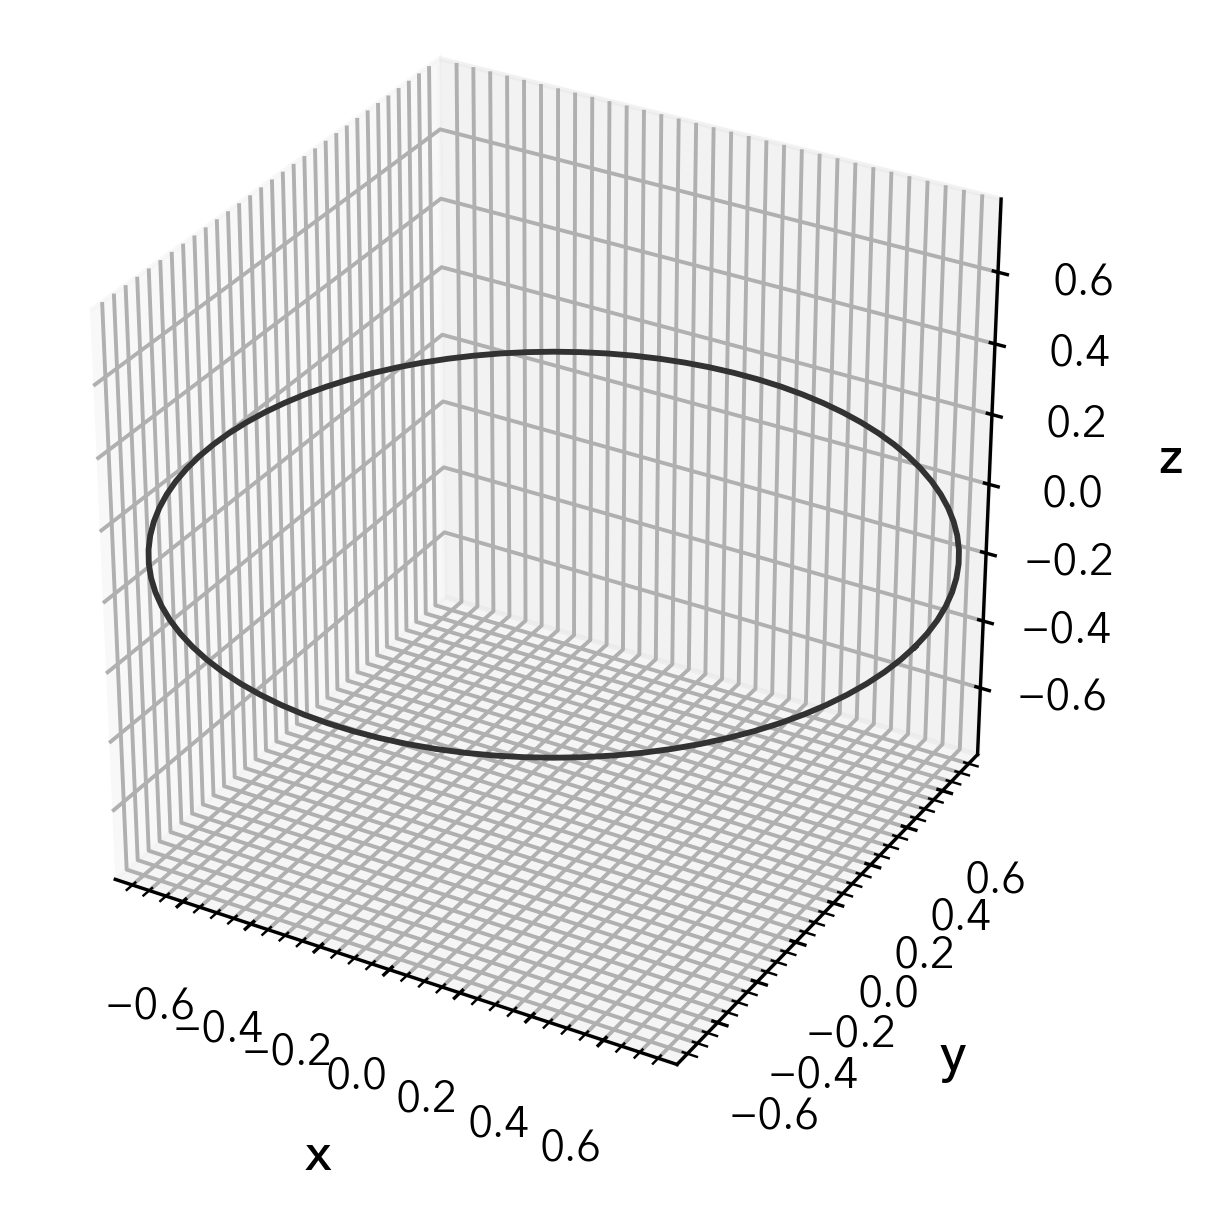
\includegraphics[width=1.0\linewidth]{./obipy-resources/zoom_3d.png}
\end{center}
\subsection{視点の角度}
\label{sec:org866ae54}
\texttt{Axes3D.view\_init()} で変更する。
パラメータの角度方向は直感の通りで、
\texttt{azim} はx軸正の向き(\texttt{y = 0} の方向)から反時計まわりの方位角、
\texttt{elev} は \texttt{z = 0} の方向からのz軸正の向きに上がる仰角。
全ての角度は単位は度で入力する。
\begin{minted}[frame=lines,framesep=2mm,linenos=true,breaklines]{ipython}
fig, ax = plot_fiducial(left=0.1)

ax.view_init(elev=15.0, azim=15.0)
# ax.view_init(elev=30.0, azim=-60.0)  # default

ax.plot(
    [1.0, 0.0],
    [0.0, 0.0],
    [0.0, 0.0],
    c=colors.black,
)
ax.plot(
    [0.0, np.cos(np.pi / 6)],
    [0.0, 0.0],
    [0.0, np.sin(np.pi / 6)],
    c=colors.blue,
)
ax.plot(
    [0.0, np.cos(np.pi / 6)],
    [0.0, np.sin(np.pi / 6)],
    [0.0, 0.0],
    c=colors.orange,
)
ax.text(
    np.cos(np.pi / 6),
    0.0,
    np.sin(np.pi / 6) / 2.0,
    'elev = 15',
    ha='right',
    color=colors.blue,
)
ax.text(
    np.cos(np.pi / 6),
    np.sin(np.pi / 6) / 2.0,
    -0.05,
    'azim = 15',
    va='top',
    ha='center',
    color=colors.orange,
)

savefig(fig, './obipy-resources/view_3d.png')
\end{minted}

\phantomsection
\label{}
\begin{center}
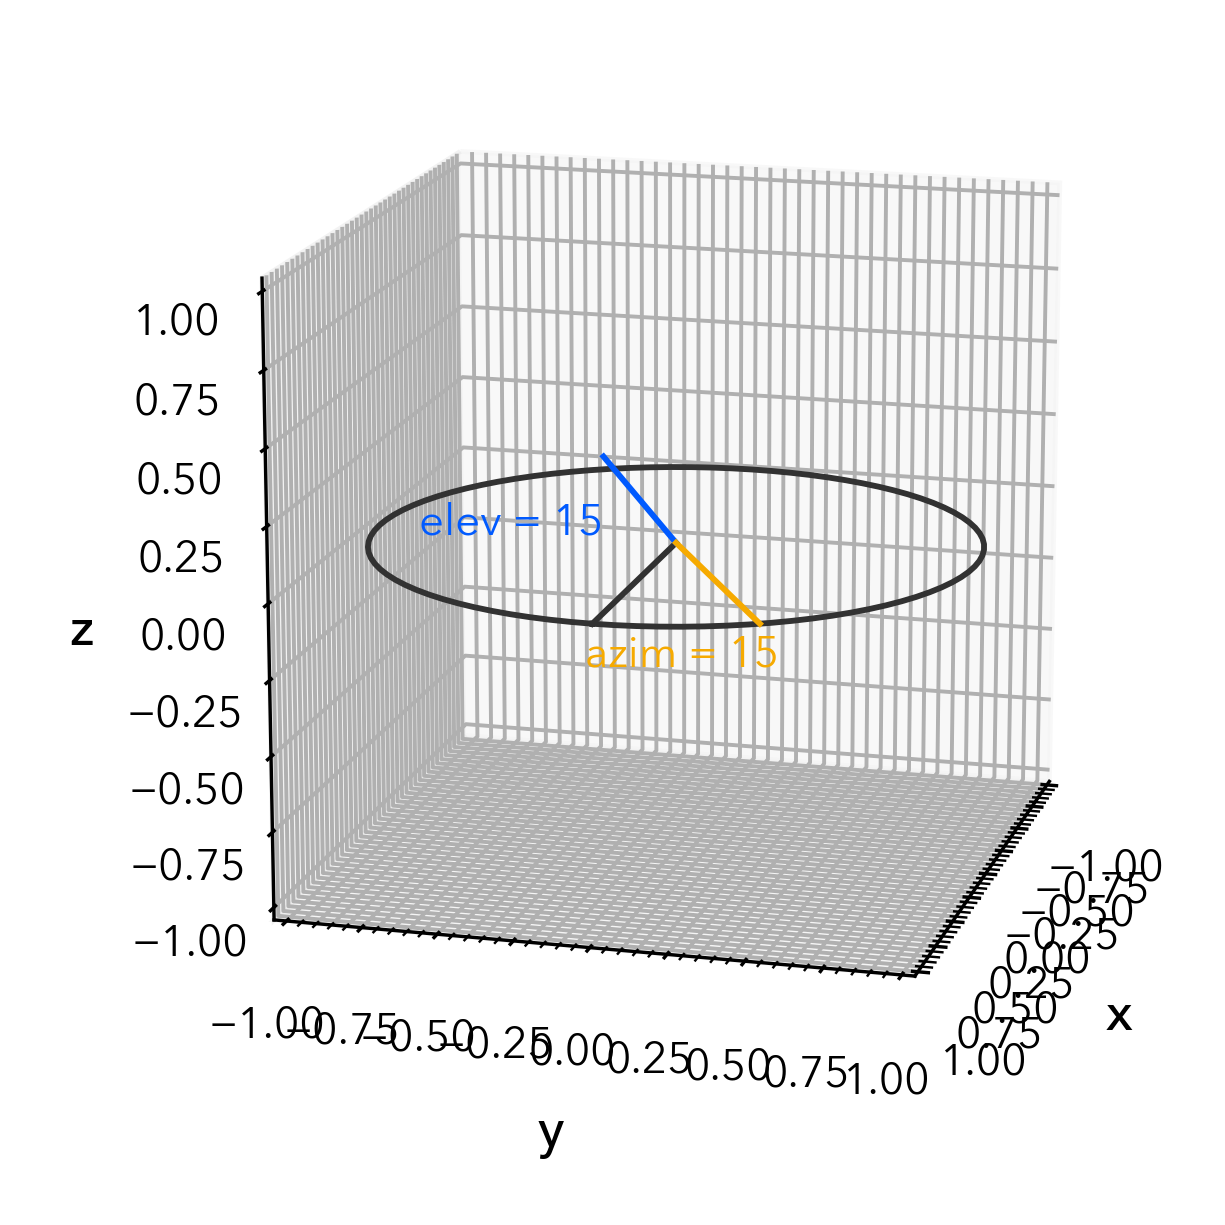
\includegraphics[width=1.0\linewidth]{./obipy-resources/view_3d.png}
\end{center}
\subsection{軸を消す}
\label{sec:orgf355797}
\begin{minted}[frame=lines,framesep=2mm,linenos=true,breaklines]{ipython}
fig, ax = plot_fiducial()
ax.grid(False)  # gridを消す
ax.xaxis.pane.fill = False  # 壁を白くする
ax.yaxis.pane.fill = False
ax.zaxis.pane.fill = False
ax.set_xticks([])  # メモリを消す
ax.set_yticks([])
ax.set_zticks([])
ax.xaxis.line.set_color((1.0, 1.0, 1.0, 0.0))  # 軸を消す
ax.yaxis.line.set_color((1.0, 1.0, 1.0, 0.0))
ax.zaxis.line.set_color((1.0, 1.0, 1.0, 0.0))
ax.tick_params(  # ラベルを消す? 消せない
    which='both',
    labelcolor='none',
    top=False,
    bottom=False,
    left=False,
    right=False,
)
savefig(fig, './obipy-resources/axis_3d.png')
\end{minted}

\phantomsection
\label{}
\begin{center}
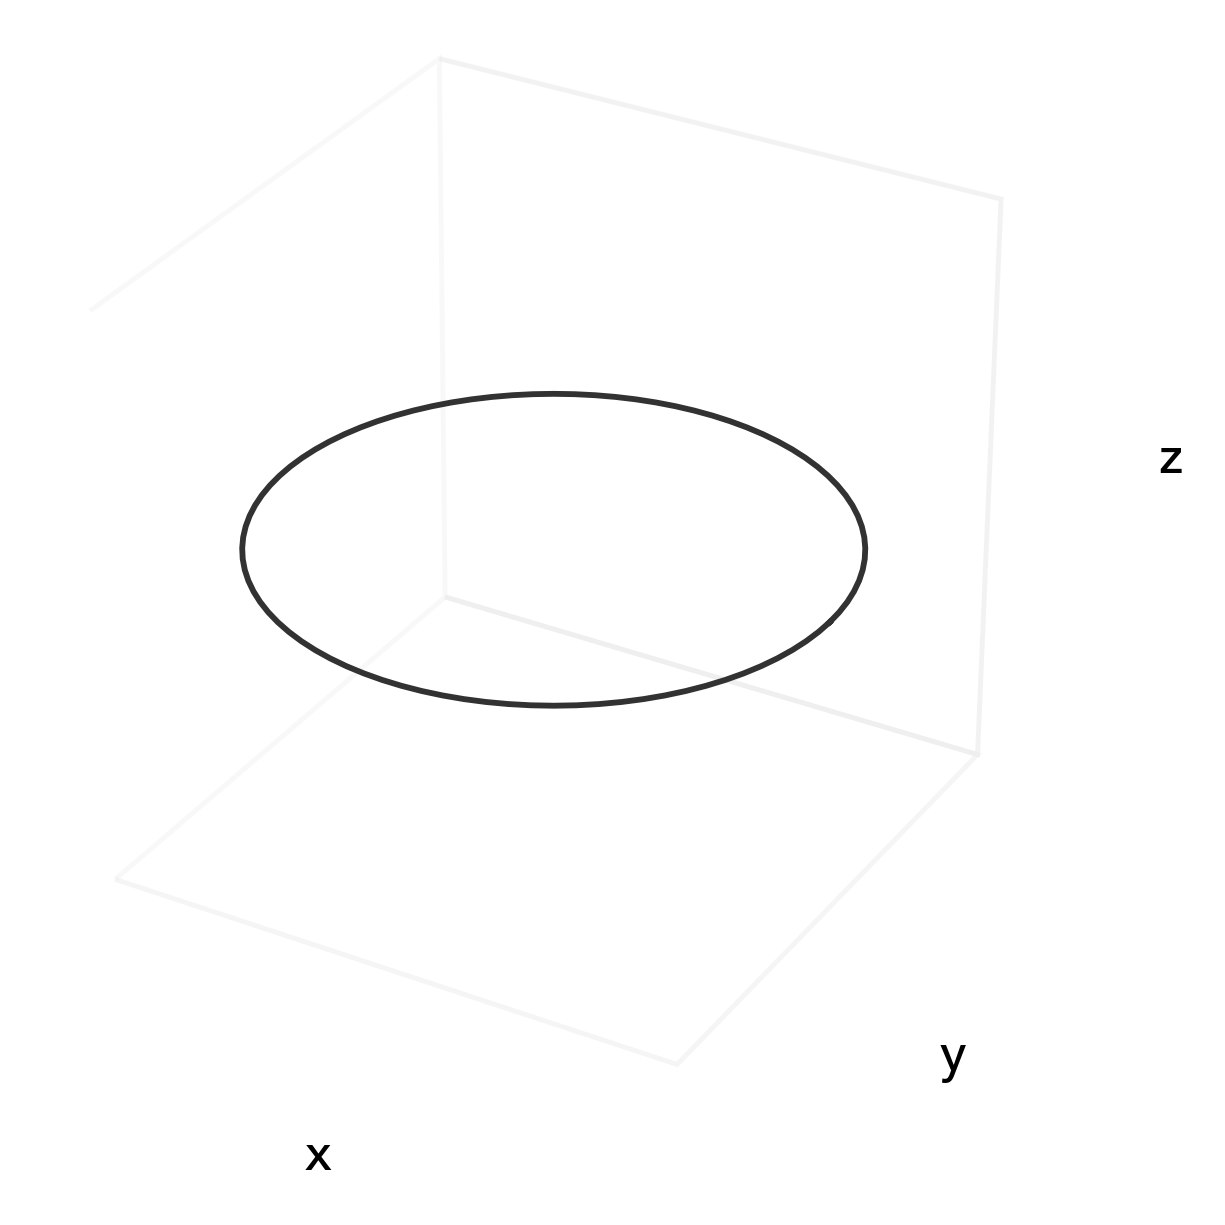
\includegraphics[width=1.0\linewidth]{./obipy-resources/axis_3d.png}
\end{center}
\subsection{軸を完全に消す}
\label{sec:org01e8338}
\begin{minted}[frame=lines,framesep=2mm,linenos=true,breaklines]{ipython}
fig, ax = plot_fiducial()
ax.axis('off')
savefig(fig, './obipy-resources/noaxis_3d.png')
\end{minted}

\phantomsection
\label{}
\begin{center}
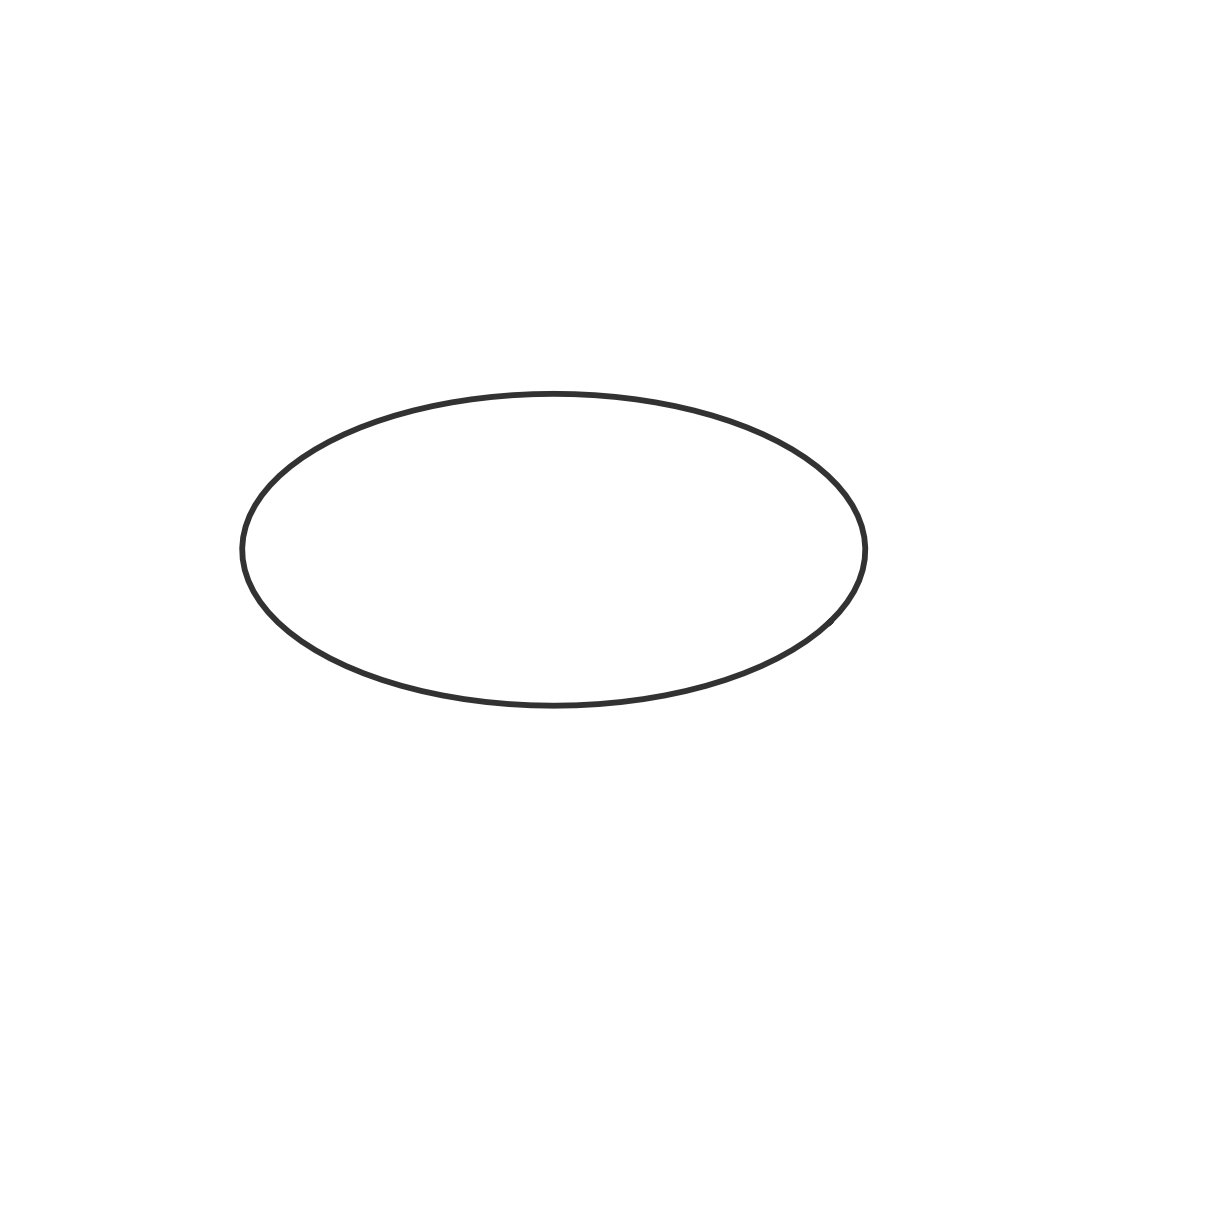
\includegraphics[width=1.0\linewidth]{./obipy-resources/noaxis_3d.png}
\end{center}
\section{プロットの工夫}
\label{sec:org00a224b}
\subsection{大量の線}
\label{sec:org400d12b}
一斉に同じ種類の線をプロットするには \texttt{art3d.Line3DCollection} を使って、返り値を \texttt{ax.add\_collection()} で加えると良い。
\begin{minted}[frame=lines,framesep=2mm,linenos=true,breaklines]{ipython}
from mpl_toolkits.mplot3d import art3d

fig, ax = plot_fiducial()
ax.axis('off')

lim = 1.3
segments = (
    ((-lim, 0.0, 0.0), (lim, 0.0, 0.0)),
    ((0.0, -lim, 0.0), (0.0, lim, 0.0)),
    ((0.0, 0.0, -lim), (0.0, 0.0, lim)),
)
linecollection = art3d.Line3DCollection(segments, colors=colors.black, lw=0.5, ls='--')
ax.add_collection(linecollection)
ax.text(lim + 0.1, 0.0, 0.0, 'x', ha='center', va='center')
ax.text(0.0, lim + 0.1, 0.0, 'y', ha='center', va='center')
ax.text(0.0, 0.0, lim + 0.1, 'z', ha='center', va='center')
savefig(fig, './obipy-resources/lines_3d.png')
\end{minted}

\phantomsection
\label{}
\begin{center}
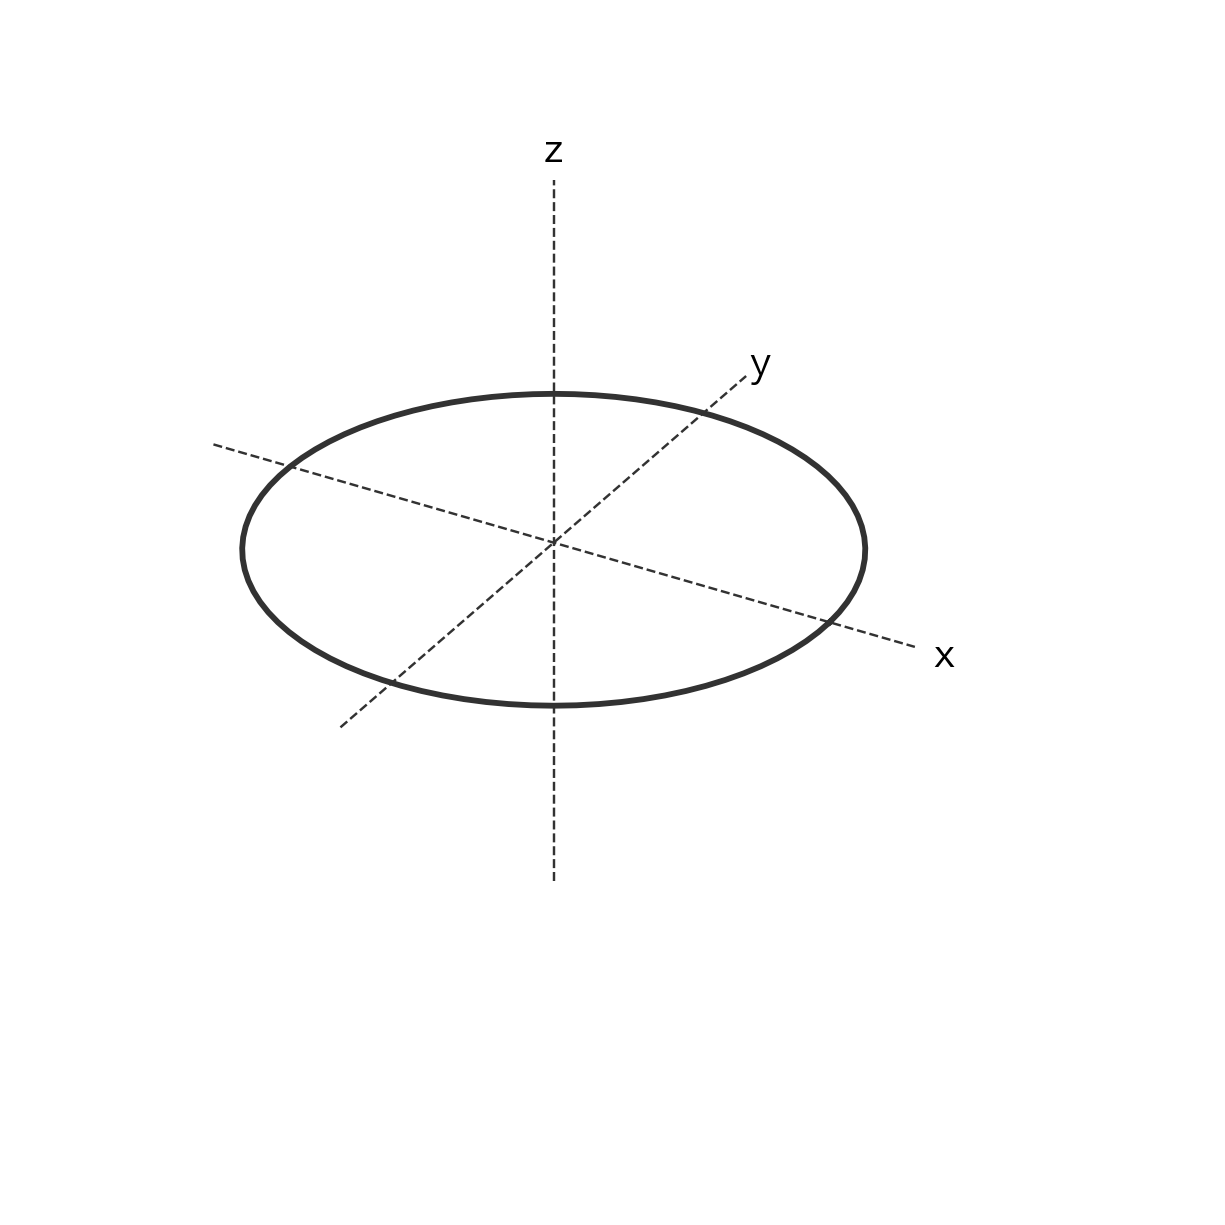
\includegraphics[width=1.0\linewidth]{./obipy-resources/lines_3d.png}
\end{center}
\subsection{光の角度}
\label{sec:org146ab7a}
光の角度は \texttt{matplotlib.colors.LightSource} で指定できる。
パラメータの角度方向は直感に反していて、
\texttt{azdeg} はy軸負の向き(\texttt{x = 0} の方向)から時計まわりの方位角、
\texttt{altdeg} は \texttt{z = 0} の方向からのz軸負の向きに下がる仰角。
つまり上からの照明は \texttt{altdeg = 90} で指定する。
\begin{minted}[frame=lines,framesep=2mm,linenos=true,breaklines]{ipython}
from matplotlib.colors import LightSource

fig, ax = plot_fiducial()
light = LightSource(azdeg=0.0, altdeg=-20.0)
# light = LightSource(azdeg=270.0, altdeg=15.0)
theta = np.linspace(1e-5, np.pi / 2.0, 10).reshape(-1, 1)
_xyz = xyz(theta, phi)

ax.plot_surface(
    *_xyz,
    color=colors.sky,
    # facecolors=facecolor,
    alpha=1.0,
    shade=True,
    lightsource=light,
)
savefig(fig, './obipy-resources/light_3d.png')
\end{minted}

\phantomsection
\label{}
\begin{center}
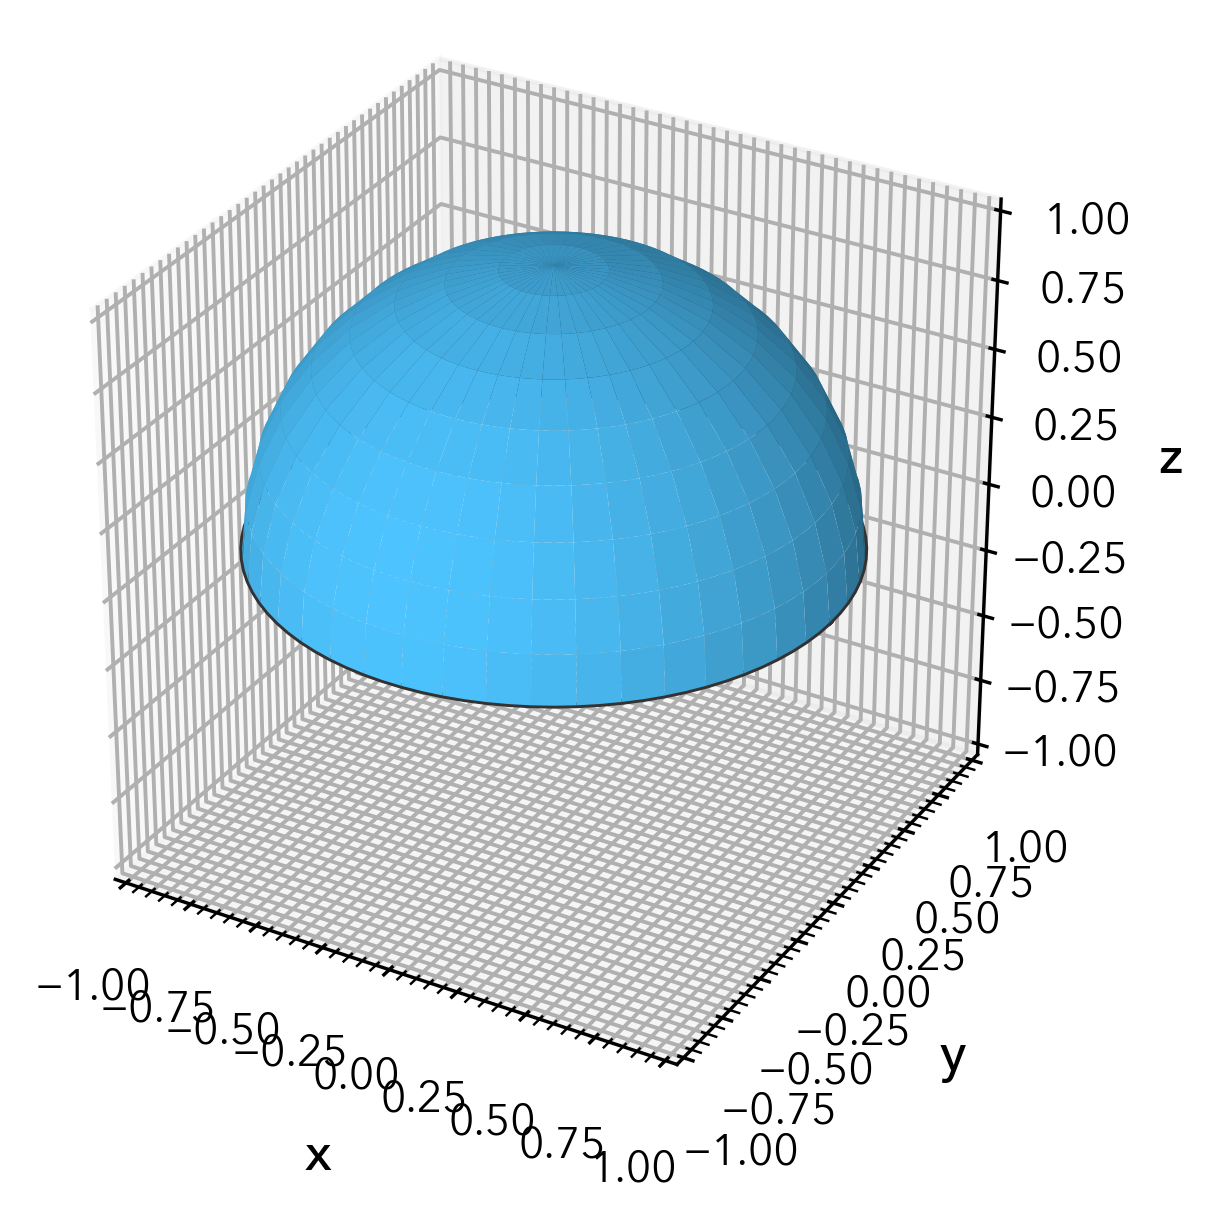
\includegraphics[width=1.0\linewidth]{./obipy-resources/light_3d.png}
\end{center}

\texttt{LightSource} は他に照明を当てた際の色の変化も指定できるが、
\texttt{Axes3D.plot\_surface()} が作る配色と異なるので注意する。
\end{document}
